%%%%%%%%%%%%%%%%%%%%%%%%%%%%%%%%%%%%%%%%%%%%%%%%%%%%%%%%%%%
% EPFL report package, main thesis file
% Goal: provide formatting for theses and project reports
% Author: Mathias Payer <mathias.payer@epfl.ch>
%
% This work may be distributed and/or modified under the
% conditions of the LaTeX Project Public License, either version 1.3
% of this license or (at your option) any later version.
% The latest version of this license is in
%   http://www.latex-project.org/lppl.txt
%
%%%%%%%%%%%%%%%%%%%%%%%%%%%%%%%%%%%%%%%%%%%%%%%%%%%%%%%%%%%
\documentclass[a4paper,11pt,oneside]{report}
% Options: MScThesis, BScThesis, MScProject, BScProject
\usepackage[BScThesis,lablogo]{EPFLreport}
\usepackage{xspace}
\usepackage{xcolor}

\title{Retrofitting defences to C++ code}
\author{Hassan Habib}
\supervisor{Nicolas Badoux}
\adviser{Prof. Dr. sc. ETH Mathias Payer}
%\coadviser{Second Adviser}
%\expert{The External Reviewer}

\newcommand{\sysname}{Retrowrite\xspace}
\newcommand{\todobox}[3]{%
	\colorbox{#1}{\textcolor{white}{\sffamily\bfseries\scriptsize #2}}%
	~\textcolor{blue}{#3} %
	\textcolor{#1}{$\triangleleft$}%
}
\newcommand{\nb}[1]{\todobox{orange}{Nicolas:}{#1}}

\begin{document}
\maketitle
%\makededication
%\makeacks

\begin{abstract}
    The \sysname tool enables lateral decomposition of a multi-dimensional
    flux compensator along the timing and space axes.

    The abstract serves as an executive summary of your project.
    Your abstract should cover at least the following topics, 1-2 sentences for
    each: what area you are in, the problem you focus on, why existing work is
    insufficient, what the high-level intuition of your work is, maybe a neat
    design or implementation decision, and key results of your evaluation.

\end{abstract}

%\begin{frenchabstract}
%For a doctoral thesis, you have to provide a French translation of the
%English abstract. For other projects this is optional.
%\end{frenchabstract}

\maketoc

%%%%%%%%%%%%%%%%%%%%%%
\chapter{Introduction}
%%%%%%%%%%%%%%%%%%%%%%

The introduction is a longer writeup that gently eases the reader into your
thesis~\cite{dinesh20oakland}. Use the first paragraph to discuss the setting.
In the second paragraph you can introduce the main challenge that you see.
The third paragraph lists why related work is insufficient.
The fourth and fifth paragraphs discuss your approach and why it is needed.
The sixth paragraph will introduce your thesis statement. Think how you can
distill the essence of your thesis into a single sentence.
The seventh paragraph will highlight some of your results
The eights paragraph discusses your core contribution.

This section is usually 3-5 pages.

%%%%%%%%%%%%%%%%%%%%
\chapter{Background}
%%%%%%%%%%%%%%%%%%%%
In this section, we will give a little bit of backround \nb{pass your check
through a spell checker e.g., grammarly} in order to understand
the experience \nb{the experience is a bit vague. Be clearer in that you want to
build up knowledge for later.}

\section{Compiler}
Computer programs can be executed in two different ways: they can be interpreted
by a software (an interpreter) or they can be compiled into machine code that can
\nb{remove word}be then be executed by the hardware. \nb{what does interpreted mean? explain a
bit more. }

In the second approach, a compiler is needed to translate the source code into binary code.
Let's have a quick overview of what is contained in a binary executable. \nb{A
bit too wordy. Something like: The resulting translation is structured inp
different sections. We will now discuss the most common format of binary executable.}

\section{Binary executable}
\subsection{ELF format}
%source man page elf
%
The dominant executable format for binary in Unix system is the ELF\footnote{Executable
and Linkable Format} format. 

An executable file respecting the ELF format must follow a certain layout. At
first it must have an ELF header followed by a program header table or a section
header table, or both. \nb{explain a bit what is the role of each section.}

\nb{Multiple tools exist that are able to}There exist multiple tools that can bes
used to display information about an ELF file. \nb{This entence doesn't bring
much. What do you want to highlight from it?}

Sometimes\nb{Why? Here you need to build up the argumentation for retrowrite}, we do not have access to the source code but we want\nb{need} to modify the
program for multiple reasons that will be listed later \nb{in Section X (use
\\autoref package and a label)}\nb{Inverse sentence, first list reason and then
what is the consequence.}. In this cas we can use
binary rewritting \nb{a technique known as }.

\section{Binary rewritting}
%%Pourquoi c'est important ???
Binary rewritting consists of modifying \nb{an executable in the absence of} without the source code an executable
\nb{while maintaining functionnality...}in a way that the program still behave as expected. It can be used for multiple
reasons as for example for program optimization, program obfuscation or as in
the case of Retriwrite\nb{use a latex command for the name} for security policy
enforcement \nb{via instr...}(instrumentation). 

\nb{This secitons is a bit out of scope here. Either introduce it earlier but
don't speak about fuzzing here. Extend a bit why we might need to retrofit
security mechanisms.}A way to test a software is by using a technique named
\textit{fuzzing}. In
order to catch bugs, one might want to compile the program with an address
sanitizer \nb{ASAN stands for AddressSanitizer}as \textit{ASan}~\cite{ASan} as they are often based on compiler instrumentation.
In the case where the source code is no longer available, the use of a binary
rewritter as for example \textit{Retrowrite}~\cite{dinesh20oakland} might be useful.
%show example of obfuscation

Binary rewritter\nb{ing or go for Binary rewritters} can be divided into two
main approach\nb{es}: \nb{lower case}Dynamic instrumetation
and static instrumentation \nb{.}

\subsection{Dynamic instrumentation}
%%executer virtuellement le programe
In this scheme, the rewritting is done while the program is executed. Usually
the binary is executed side by side with the rewritter engine. In order
to analyse \nb{Not only analyze but also interact} the binary during the execution, the rewritter might use the OS's
primitves as the PTRACE API in Linux for example.  Only the parts executed can
be analysed and rewritten so they can focused and the most important
part\nb{This last sentence doesnt make sense. What are the advantages, disadv?}.

\subsection{Static instrumentation}
\nb{Contrariy to dynamic ...}Here, the rewritter operates on binaries stored in
persistent \nb{at static time } memory
(executables that are not being run). In\nb{It} outputs a new binary executable that
corresponds to the initial executable but rewritten. \nb{Uppercase}\nb{This (to
be conssitent with the previous sentnece)}these executables have the
advantage of being almost as fast as the original executable that would have
been compiled for instrumentation.\nb{why?}



\subsection{Steps in binary rewritting}
Both dynamic and static instrumentation follow four main steps:
\begin{enumerate}
    \item Parsing:
        This step consist of obtaining the instruction stream from the binary
        and pass it to a disassembler.
        %elaborate
    \item Analysis:
        %elaborate
        This part consists of gaining as much information as possible \nb{bei
        consistent in the use of . (dots)}\nb{Which kind of information?}
    \item Transformation:
        %elaborate
        Here, we must find all the locations where  code \nb{do we always add
        code? Why not remove? Also don't use code but instrumentation}must be added. 
    \item Code generation:
        %elaborate
        Here \nb{redundant} we have to make sure that adding the code does not modify the
        behaviour of the executable \nb{avoid parenthesis. Rework the sentence}(the modified code must run as the
        original). There are multiple techniques for this part. \nb{Code gen is
        mostly going back from the lifted language (AR; dissabled  instructions)
    to machine code again. }
\end{enumerate}
%add a figure
\begin{figure}[h]
    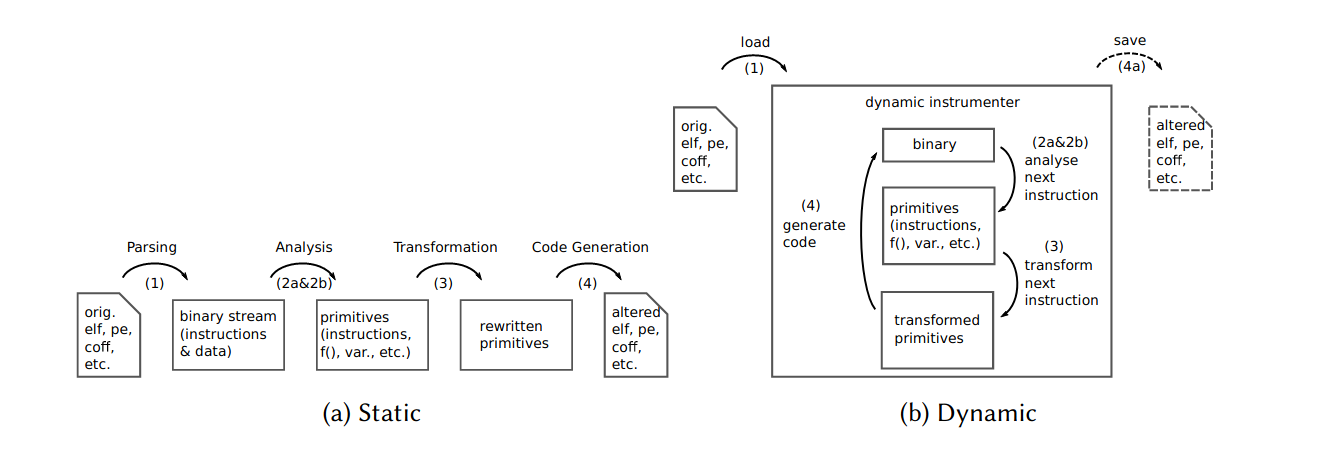
\includegraphics[width=\linewidth]{required_steps.png} 
    \caption{Required steps for binary rewritting\nb{Make two figures. Add
    refernce to the figure in the text. The figure shold help understand
    something and not just be there for beauty}}
    \label{fig:steps}
  \end{figure}
\subsection{Code genreation techniques}
\nb{If I understood it correctly trampoline are  more a transformation technique than a codegen one.}
There are multiples techniques for the transformation and code generation
parts. The simplest techniques is called \textit{Trampoline}. All new code are
added in new sections in the binary. Branches are then added to redirect to the
right location after an instrumentation point. In this techniques, no reference
or branches are broken. \nb{Why do we need to do that. Eplain the challenge of
fixed refernec earlier.}

Another technique is named \textit{Direct}. This is one of the oldest
technique. Here the code is simply overwritten. We have to make sure to reajust
every braches\nb{typo} and references\nb{and is hard? why?}.


The technique used by \textit{Retrowrite} is called \textit{Symbolization}. It
consist\nb{s} of transforming the binary into an assembly text file. It transforms
all references constants into assembly labels. Then\nb{,} many tools can instert\nb{typo}
instrumentation into the reassembled file. Unlike the trampoline technique,
this method is defined as being \textit{zero-overhead} \nb{why? Speak about the
overhead in each section!}
%add example of symbolization

\section{Retrowrite}
%link to paper
Retrowrite~\cite{dinesh20oakland} is a binary rewritter developped by HexHive. It uses the
symbolization technique by generating re-assembleable assembly. Their approach
is sound by construction because they use relocations, PC-relative addressing,
and recovered control flow to determine reference constants and symbolize
them\nb{Nice sentence, but you did not eplxain me these terms earlier!}\nb{Whyi
does t makes it sounds}.
It uses \textit{Capstone} as a disassembler and \textit{pyelftools} as a binary
parser.

\nb{Speak a bit about HexType or other C++ securtiy tehcnique we looked at the start}


%%%%%%%%%%%%%%%%
\chapter{Goal}
%%%%%%%%%%%%%%%%
As stated in their paper~\cite{dinesh20oakland}, \textit{Retrowrite} was
firstly designed to support Linux x86-64 PIC binaries that were written in the
\textit{C Programming Language}.
The main obstacle for adding support for \textit{C++} is that \nb{remove word}the symbolization
for \nb{of}C++ exception handlers is \nb{not yet supported} missing. \nb{Dont
start a sentence with but}But multiple works were done in order to
add support for C++ as it can be seen in the \textit{Retrowrite} repository
~\cite{gitCommit} \nb{.} \nb{Discuss what was the status when you started the
project. Why is it interesting etc...}


\nb{We are missing a page about challenges. This should be much longer.}

\section{Task}
The task was to test a large number of packages from the \textit{Debian}~\cite{debian} distribution.
Debian being a widely used distribution within the Linux community, \nb{too verbose}we thought
it would be a good idea to use it as a source. We first tested the most used
programs and then we have another list containing a list of programs without a
particular orders\nb{again, shorten the sentence. Do we actually need to speak
about that here?}. From the results obtained, we try to see if Retrowrite can
indeed rewrite programs written in C++ and we also try to see where it has
trouble. Then we chose some programs where we try to rewrite the binaries with retrowrite
and we try to see where exactly the program crashes. \nb{This whole paragraph
should be part of the above one where you gently explain why we need more
testing and why we wanted to test on this code (diversity of C++ coding patterns
for example). and why not Chromium (too big, not handled by Rretrowrite)}


%%%%%%%%%%%%%%%%%%%%%%%%
\chapter{Implementation}
%%%%%%%%%%%%%%%%%%%%%%%%
All the scripts used can be found in the github\nb{Uppercase G} 
\href{https://github.com/ha2san/debian_docker/tree/main/scripts}{repository}~\cite{repo}\nb{better
cite it at the end of the section. This breaks the flow of the reader}.

The main script is \textit{clone.sh}.It will start several containers which will
each take care of one package. This script also takes care of running the
command that will prepare the results.

\section{Docker}
The first decision was to test \textit{Retrowrite} in
\textit{docker}~\cite{merkel2014docker} containers. This allows us to emulate
debian \nb{be consistent with D d } on
any machine. Each container will execute \textit{entrypoint.sh} on a specific package. The
binaries available from the command \textit{apt install}~\cite{apt} are stripped, so
we had to download the source code and compile the program ourselves. Then the
\nb{main task is just extra words without any benefits}main task was to run the
program with the argument "\textit{--help}" \nb{Why help, this should be
discussed in the previous section}and
compare the exit code with the recompiled program from the assembly file
re-assambled by retrowrite. The programs are then sorted according to their
output code.

\section{Linking}
One problem encountered was recompiling the
assembly files by linking them to the correct shared-libraries. To do so, a 
script was written called \nb{use markup} flib.sh which takes as argument the original binary
file. It will then return, using the command "ldd"\cite{ldd} the list of
libraries to link. 

\section{List of packages}

Having obtained a list of packages from the Debian distribution
\cite{sourcePackage}, we needed a way of filtering to only obtain
a list of packages written in \textit{C++}. To do this, we use the script
\textit{filter\_c++\_packages.sh}. It will simply look in the information given
in \textit{apt show}~\cite{apt} if the package was written in \textit{C++} or
not. 

\section{Filtering the result}
When the docker containers have finished executing their commands, the
\textit{result\_count.sh} script will be executed. This script takes care of searching
and sorting the results by arranging them and putting them in a new folder.
%explain the categories when it is more clear

\section{Three programs}
We have chosen three programs that we will test manually and try to find out
where the errors may come from. The three programs are
flameshot~\cite{flameshot}, bitcoind~\cite{bitcoind} and
fish-shell~\cite{fish}.\nb{why these}


%%%%%%%%%%%%%%%%%%%
\chapter{Evaluation}
%%%%%%%%%%%%%%%%%%%

%show table or graph about popular packages
%show table or graph about all tested packages
%show errors with three tested program
%interpret result


%%%%%%%%%%%%%%%%%%%%%%%
%\chapter{Related Work}
%%%%%%%%%%%%%%%%%%%%%%%
%
%I can cite other rewritter.



%%%%%%%%%%%%%%%%%%%%
\chapter{Conclusion}
%%%%%%%%%%%%%%%%%%%%

In the conclusion you repeat the main result and finalize the discussion of
your project. Mention the core results and why as well as how your system
advances the status quo.

\cleardoublepage
\phantomsection
\addcontentsline{toc}{chapter}{Bibliography}
\printbibliography

% Appendices are optional
% \appendix
% %%%%%%%%%%%%%%%%%%%%%%%%%%%%%%%%%%%%%%
% \chapter{How to make a transmogrifier}
% %%%%%%%%%%%%%%%%%%%%%%%%%%%%%%%%%%%%%%
%
% In case you ever need an (optional) appendix.
%
% You need the following items:
% \begin{itemize}
% \item A box
% \item Crayons
% \item A self-aware 5-year old
% \end{itemize}

\end{document}
